\documentclass[twocolumn]{article}
\usepackage{graphicx}
%\usepackage{fancyhdr} 
%\usepackage{fancybox}
\usepackage{float}
\usepackage{listings}
\usepackage[colorlinks=true,urlcolor=black,linkcolor=black]{hyperref}
\usepackage[margin=1.0in]{geometry}
\usepackage{multicol}
%\pagestyle{fancy}

%redefines subsections with letters instesad of numbers
%\renewcommand{\thesubsection}{\thesection.\alph{subsection}}

% Center Image Command
\newcommand{\centerimage}[3]{
\begin{figure}[ht!]  
\begin{center} #1
\caption{#2}
\label{#3}
\end{center}
\end{figure}}

\title{\textbf{Branch Predictor and Branch Target Buffer} \\
ECE 486/586 Final Project }
\author{Eric Krause \hspace{1.4in} Bradon Kanyid\\
\url{ekrause@pdx.edu} \hspace{1in} \url{bradon@kanyid.org}}

\begin{document}
\twocolumn[
  \begin{@twocolumnfalse}
    \maketitle
    \begin{abstract}
      ...
    \end{abstract}
  \end{@twocolumnfalse}
]
\textbf{Keywords:} Branch Prediction, Branch Target Prediction, Simulation, Heuristics, ISA, 0xBEEFA55

\section{Background Information}
For this project, we were required to duplicate the tournament branch predictor used in the Alpha 21264 processor, then design a corresponding branch target predictor.  The size budget for both parts of the project (Alpha predictor and branch target predictor) was 8Kb.  The entire system was then tested against 20 instruction traces from an unknown ISA. \\\\
There were additional constraints as well: all table sizes had to be powers of 2, multiplying or dividing by numbers other than powers of two was not permitted, and tables with associativity $\ge$ 8 incurred a penalty equal to the size of the table.\\\\
Our branch predictor was modeled after the predictor described in R. E. Kessler's paper on the Alpha 21264 microprocessor.  Figure \ref{alpha} shows our implementation of the Alpha predictor.  One key difference between our implementation and Kessler's is that our predictor is only called on conditional branches, not all instructions.\\\\\section{Branch Prediction}\centerimage{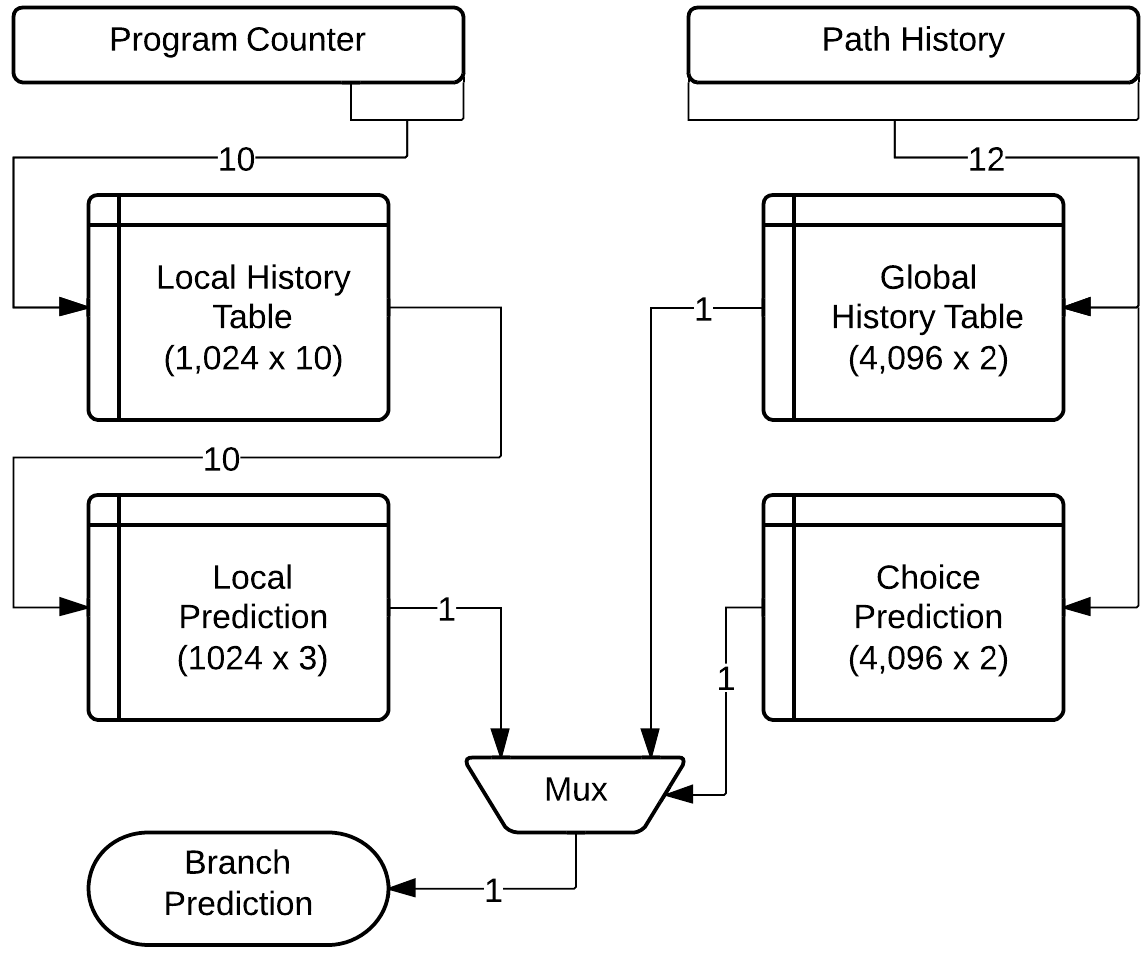
\includegraphics[width=\columnwidth]{alpha.png}}{Alpha Predictor}{alpha}\centerimage{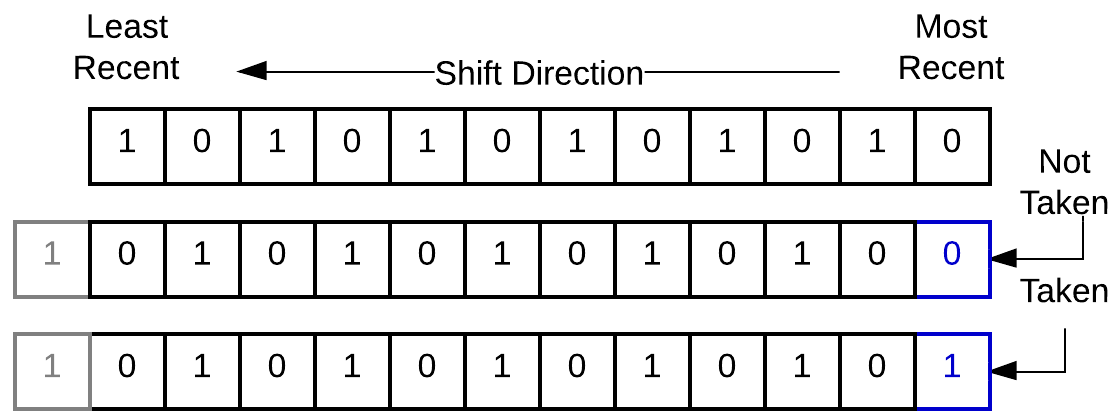
\includegraphics[width=\columnwidth]{phistory.png}}{Path History Shift Register}{phistory}
The Alpha predictor is a tournament predictor, meaning that it makes multiple predictions (based on the global and local histories) and then chooses between the prediction that has  been the most accurate, based on the path history.  The path history (illustrated in figure \ref{phistory}) is a shift register that maintains a history of the most recent 12 conditional branches by shifting in 1 or 0 for taken or not taken branches respectively.\\\\
Path history is used as an index into the 4,096-entry choice prediction table, which maintains 2-bit saturating counters at each location which indicate whether--given the current path history--the local or global prediction has been more accurate.\\\\  
The global history table is also indexed using the path history, and consists of 4,096 2-bit saturating counters indicating whether--given the current global path history--the next branch is likely to be taken or not taken.\\\\
The local history table is indexed by the least significant 10 bits of the program counter.  Each entry in the local history table is a 10-bit path history for instructions (in our implementation, \textit{conditional branches}) with the same least significant 10 bits.  These local histories are used as indices into the local prediction table, which consists of 1,024 3-bit saturating counters indicating whether--given a local path history--the next branch is likely to be taken or not taken.\\\\
The strength of this design is that it can take advantage of branch patterns occurring within working sets of various sizes, with the local history being more useful with small working sets, and the global history being more useful for large working set.  

A few implementation details were absent from Kessler's paper, so assumptions were made to create the most accurate predictor possible.  These fell into three categories:  Initialization values for the saturating counters and path history, under what conditions updates should occur, and how to handle unconditional branches (jumps).

\subsection{Initialization Values}
\subsection{Conditional Updates}
\subsection{Unconditional Branches}

\section{Branch Target Prediction}
In a high-performance processor, simply predicting whether a branch is taken or not taken accurately is not enough to eliminate pipeline stalls.  If taken, the destination address of the branch must also be predicted so that instructions beginning at the target address can be speculatively executed. 
 
\subsection{Development History}
Our development process was much like a small weasel--somewhat iterative, yet dynamic and highly agile. 

\subsubsection{Direct Mapped}
\subsubsection{Relative Offset Table}
\subsection{Final Design}
\subsubsection{Dynamic Objects}
\subsubsection{Main Cache}
\subsubsection{Return Address Stack}
\subsubsection{Victim Cache}
\section{Size Budget}
\section{Testing Methodology}
\section{Results}
\section{Conclusion}
\appendix
the codes
\end{document}